\section{Prototype Validation}\label{prototype_validation}

\subsection{Testing Framework}\label{testing_framework}
Validating a software using property based testing requires that a property is
expressed in some target programming language. This property can be then
checked by generating random inputs for the property and testing whether it
holds for them. Cardano is implemented in Haskell, so we will be expressing our
properties in Haskell, and using \lstinline{QuickCheck} as our property based
testing library.

A quintessential example of a property is that reversing a list twice should
yield the original list. This can be readily expressed as follows:

\begin{lstlisting}
	prop_reverse :: [Int] -> Bool
	prop_reverse xs = reverse (reverse xs) == xs
\end{lstlisting}

Testing this property requires that the test program has a way to generating
random integers (\lstinline{Int}).

When a property fails, a \emph{counterexample} is produced. It is very
important that said counterexample is small since this aids the developers in
understanding the cause of the problem. For instance, consider
\lstinline{prop_reverse} above failing due to a wrong implementation of
reverse, and giving as a counterexample a list of 1000 elements. If the problem
can be reproduced with a list of three elements, then this would be highly
preferred. To enable \lstinline{QuickCheck} to give minimal counterexamples
we need to provide a \emph{shrink function} for our data types. A shrink
function basically determines for a given value the ways in which it can be
shrunk. Thus a good counterexample depends on good shrinking.

Another important aspect of property based testing is the degree of coverage
our tests have. For instance, if we test a property of integer lists with only
small integer values we might miss to uncover violations to this property
caused by very large values. Therefore, besides testing our properties when
doing property based test it is important to \emph{test the coverage of the
	generators}. Luckily \lstinline{QuickCheck} provides good support for
writing
and performing these tests. So for instance, we can write tests that state that
10\% of our test cases should consist of lists with at least 5 large numbers.

So to summarize, using property based testing as validation methodology
requires to:

\begin{itemize}
	\item Express the properties in Haskell.
	\item Write generators for the input data.
	\item Write shrink functions for the input data.
	\item Write coverage tests for the generators.
\end{itemize}

% Expressing the properties of the update system...
%
% ... we do this in term of traces.
Cardano is divided intro three main components:
\begin{enumerate}
	\item Network: which takes care of communication between nodes and clients
	(such as wallets).
	\item Consensus: which runs the consensus algorithm. This layer communicates
	with the ledger layer.
	\item Ledger: which encodes the logic for determining which transactions are
	valid.
\end{enumerate}

The bulk of the update system will be implemented in the \emph{ledger layer} of
Cardano.

The ledger layer API consists of a set of state transforming functions: this
is, given an initial ledger state and some data-value (like a transaction or a
slot-number), the functions in this API return either an error (if the data
could not be applied in that state) or the state resulting from applying the
given value to the given state.

Given that the ledger API is organized as a set of state transforming
functions, we can characterize \emph{any} evolution of the ledger state as an
interleaved sequence of state and actions: such sequence starts with some
initial state, it is followed by a sequence of pairs of action and ensuing
state. We call such sequence a \emph{trace}.

Since we can characterize the behavior of the ledger in terms of set of traces,
we can then express certain properties of the update system in terms of
properties on traces. Thus, when testing the properties of the update system we
will write:

\begin{enumerate}
	\item Update system (ledger) trace properties.
	\item Generators for these traces.
	\item Shrink functions for traces.
	\item Coverage tests on traces.
\end{enumerate}

% Why properties of ledger traces are transferable to properties of the
%blockchain?
Note that properties that hold on (ledger) traces are transferable to the whole
blockchain system since the consensus layer relies on the ledger to validate
transaction, which means that in the blockchain we will only see sequences of
transactions (traces) that are allowed by the ledger.

\begin{figure}[h!] %[H]
	\centering
	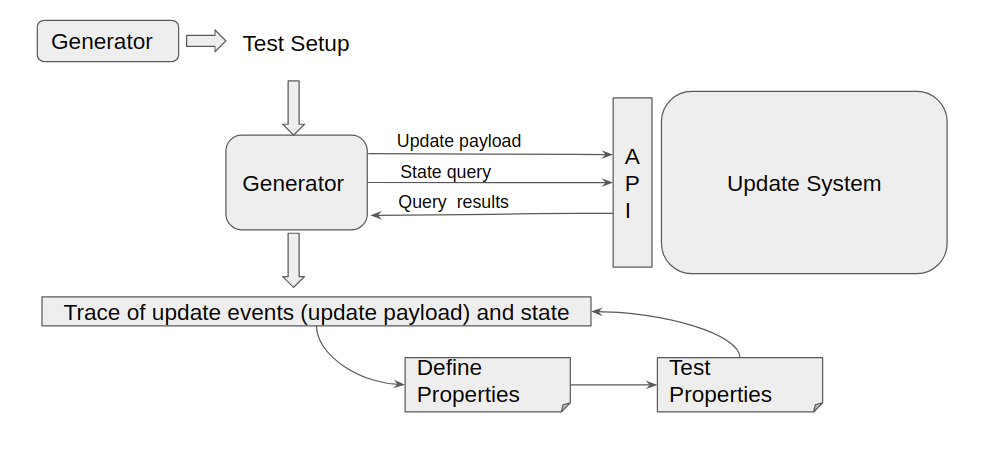
\includegraphics[width=0.8\columnwidth,
	keepaspectratio]{figures/testing_framework.png}
	\caption{The testing framework for software updates.}
	\label{fig:testing_framework}
\end{figure}

In figure \ref{fig:testing_framework}, we depict a high-level view of our
testing framework. We can see the generator generating various test setups,
which are fed into the main generator, which produces all the relevant update
events (update payload). For each such payload the update system API is
invoked, in order to handle it. The update system consumes the update payload
based on the implemented update logic and consequently updates the
\emph{update
	state}. The main generator
queries this state and records it in a trace along
with the update payload generated in a chronological order. Finally, we define
conditions (i.e., properties) over this trace of events, which constraint what
state transitions are valid and with what update events this transition should
take place. These conditions essentially form our validation criteria.


\subsection{Validation Criteria}\label{validatioin_criteria}
\subsubsection{Requirements driven validation criteria}
One of the most important goals of the Cardano blockchain is to enable
\emph{decentralized governance}. This is, the decisions
for the evolution of the system should be made collectively by the Cardano
stakeholders (a.k.a. the Cardano community) and the costs of evolving the
system (e.g research and development)
should also be paid
by them, via a Treasury system that is collectively funded. The Cardano
decentralized
software update system developed in
the context of PRIViLEDGE is undoubtedly a center piece in this decentralized
governance puzzle.

Clearly, the design of the software update system is requirements-driven. The
requirements are ultimately posed by the Cardano community and are eventually
conveyed to our team via various internal (to IOHK) stakeholders; for example
the Cardano Product Management. In deliverable \emph{D1.1 Requirements and
	Interface Design} \cite{priviledge_d11}, we have described an initial set 
	of 
requirements. Since
then, this set has been discussed internally, has matured and been enhanced
and currently has been aggregated to eight \emph{vision statements} that
capture the essence of the to-be update system. We briefly outline these
high-level
requirements next. These will be our main driver for defining the
validation criteria\footnote{In the rest of this text we will use the terms
	''validation criteria'' and ''properties'' interchangeably.} in the rest of
this section.

\subsubsection{The Cardano software update system vision
	statements}\label{sec:vision_statements}
\begin{itemize}
	\item[\textbf{Open Participation Enabled}] Anyone who can submit a common
	transaction should be able to submit an update proposal and vote for an
	update proposal.
	
	\item[\textbf{Decentralized Decision-Making Enabled}]  All major decisions
	typically made by central authorities (e.g., code maintainer, software
	owner etc.)
	should
	be made
	collectively by the community via a voting mechanism: a) What proposal will
	move forward? b) Do we accept the submitted implementation? and c)
	will the changes be activated?
	
	\item[\textbf{Protocol-Driven}] The update mechanism should be an on-chain
	protocol driven process: Not
	based on informal discussions (social consensus\footnote{Although this is
		also a very useful preparatory step to utilize along with the update
		protocol.}), but based on a protocol
	with specific security guarantees; a protocol that will leave behind an
	immutable (on-chain) trace of events
	
	\item[\textbf{Transparent and Auditable}] Anybody should be able to answer
	\emph{when}, \emph{why} and \emph{how} the system has evolved the way it
	has. The evolution history of the system should be open to everyone and
	form a globally-consistent tamper-evident public release log.
	
	\item[\textbf{Secure Activation Enabled}] The activation of changes on the 
	blockchain system should be resilient to chain-splits and ensure a secure 
	transition from the previous version of the consensus protocol to the new 
	one. We need to formally define what is a \emph{secure
		activation} and propose a protocol that enables such an activation.
	
	\item[\textbf{Performant and Scalable}] The update mechanism should have a 
	minimal impact on the transaction throughput and size of the underlying
	blockchain. Moreover, the update mechanism should be scalable to thousands
	(or even
	millions) of participants.
	
	\item[\textbf{Metadata-Driven Update Logic}] All updates are not the same
	(criticality,
	impact on the system, time to deploy etc.). We should enable a
	metadata-driven update policy (voting periods length, activation priority,
	deployment window etc.). This update policy should efficiently handle
	priorities, version dependencies, update conflicts and emergencies, in
	order the system to always be at a consistent state.
	
\end{itemize}


\subsection{Open participation}\label{sec:open_participation}
The \emph{open participation requirement} states that anyone who can submit a
common transaction should be able to submit an \emph{update 
	payload}\footnote{An \emph{update payload} refers to an update 
	proposal(SIP/UP), a 
	vote for an update proposal, a signal for upgrade readiness and in general 
	any 
	event that relates to the update protocol and is stored in the 
	transaction's 
	metadata called \emph{payload}.}, provided that such
payload is valid according to the protocol. The update payload refers to any of
the following data:
\begin{itemize}
	\item SIP commitments, revelations, or votes; or
	\item implementation commitments, or revelations (see about commit-reveal 
	scheme in section \ref{sec:su_lifecycle}), votes, or endorsements (i.e., 
	upgrade readiness signals).
\end{itemize}

We consider that the system satisfies the open participation requirement when
the following validation criteria are met:
\begin{itemize}
	\item Authorship of proposals should be preserved.
	\item Valid proposals' commitments are not rejected.
	\item Valid proposals' revelations are not rejected.
	\item Valid proposals' votes are not rejected.
	\item Valid implementation endorsements are not rejected.
\end{itemize}


These validation criteria ensure that any update event (i.e., update payload)
can be submitted to the blockchain, without it being rejected, as long as: a)
it is valid and b) it has payed the necessary fees.  They are detailed in the
next section, along with the
\emph{validity conditions} for each type of update payload. Therefore
conditioned to
these constraints anyone can participate.  It is important to
note that in these validation criteria, we will not be
mentioning fees. The fees are checked by the UTxO layer. We assume that the
payload passed to the update system will be part of a transaction that
spends at least the fees that the update payload must pay (which is determined
by the UTxO layer\footnote{Our prototype will be ''plugged into'' the Cardano
	ledger layer. This layer includes an UTxO layer that handles all this ''UTxO
	logic''}.)

\subsubsection{Authorship of proposals should be
	preserved}\label{vc:proposals_authorship}

The protocol should prevent proposal authorship of proposals from being stolen.
To this end, the protocol enforces a commit-reveal scheme for proposals.
This validation criterion validates that the commit-reveal scheme indeed works
correctly.

Proposals can be revealed only after a corresponding commitment is 
\emph{stable} on
the chain. A commitment should contain the commitment payload, as well as the
verification
key (i.e., public key) of the author, say $vk$, that submitted 
the commitment. The commitment payload
should be of the form:
\begin{math}
	H (salt || vk || H (proposal))
\end{math}
, i.e., A salted commitment to the Update Proposal (either a SIP, or a UP) hash
as well as the public key of the issuer, where $H$ is a cryptographic hash
function.

If the verification key of the commitment author is part of the information 
stored
in the commitment, then the protocol can ensure that the commitment author and 
the
revelation authors are the same. To see why this is the case, consider the
following analysis. A commitment submission comprises:
\begin{itemize}
	\item the commitment payload, which is of the form $H (salt_0 || vk_0 || H
	(proposal_0))$
	\item the verification key of the author, say $vk_1$
	\item a signature of the payload by $vk_1$
\end{itemize}

The corresponding revelation submission comprises:
\begin{itemize}
	\item $proposal_1$ metadata %$H (proposal_1)$
	\item $salt_1$
	\item $vk_2$
\end{itemize}

We assume that from the submitted proposal metadata we can retrieve the actual 
proposal. So if we compute $H(salt_1 || vk_2 || H (proposal_1))$ and this is 
equal to
$H(salt_0 || vk_0 || H (proposal_0)$, then it must be the case that $vk_0 =
vk_2$, and since we also checked that $vk_1 = vk_2$, we have that $vk_0 =
vk_1$. Of course we assume that $H$ is a collision resistant hash function.

Therefore for this validation criterion we have the following \emph{validity
	condition}:

\begin{equation}\label{eq:commit-reveal-match}
	H(salt_1 || vk_2 || H (proposal_1)) = H(salt_0 || vk_0 || H
	(proposal_0) \land
	vk_1 = vk_2
\end{equation}

\subsubsection{Valid proposal commitments are not
	rejected}\label{vc:commits_not_rejected}
In this validation criterion, we ensure that no proposal (SIP or
Implementation)
commitment can be rejected by the update system, unless the following validity
condition is violated:
\begin{itemize}
	\item the commitment signature verifies and
	\item the commitment has not been already submitted.
\end{itemize}

If both of the conditions above hold, then the commitment should be accepted. If
any of these two conditions is violated, then the commitment should be rejected.
Note
that in particular this means that the system allows an implementation 
commitment
to be submitted at any time, as long as they are valid. This is true even in
the case, where an implementation commitment does not match a previously 
approved
SIP. Indeed, commitments are basically hashes so the system does not have the
possibility of performing any semantic check on the commitment.

In summary, in all generated traces, and for all proposals'
(SIPs/UPs) commitments submitted to the blockchain, no commitment should be 
rejected,
unless the said validity condition is violated.


\subsubsection{Valid proposal revelations are not
	rejected}\label{vc:revelations_not_rejected}
In this validation criterion, we ensure that no proposal (SIP or
Implementation) revelation can be rejected by the update system, unless the
following validity condition is violated:
\begin{itemize}
	\item the revelation matches a previously submitted commitment (see 
	condition
	\ref{eq:commit-reveal-match}), and
	\item the matched commitment is stable on the chain
\end{itemize}

If both of the conditions above hold,  then the revelation is valid and should
be accepted. If any of these two conditions is violated then the revelation 
should
be rejected.

In summary, in all generated traces, and for all proposals'
(SIPs/UPs) revelations submitted to the blockchain, no revelation should be 
rejected,
unless the said validity condition is violated.

\subsubsection{Valid proposal votes are not 
rejected}\label{vc:votes_not_rejected}
In this validation criterion, we ensure that no vote for a proposal (SIP or
Implementation) can be rejected by the update system, unless the
following validity condition is violated:
\begin{itemize}
	\item the signature of the vote is valid and
	\item the vote refers to a proposal known to the system and
	\item the voting period for the proposal is open
\end{itemize}

If all of the conditions above hold, then the vote is valid and should be
accepted. If any of these conditions is violated, then the vote must be
rejected.

In summary, in all generated traces, and for all proposals'
(SIPs/UPs) votes submitted to the blockchain, no votes should be rejected,
unless the said validity condition is violated.

\subsubsection{Valid implementation endorsements are not
	rejected}\label{vc:endorsements_not_rejected}

In section \ref{sec:su_lifecycle}, we have described that an \emph{endorsement} 
is a signal of upgrade readiness issued by the block producers. In this 
validation criterion, we ensure that no endorsement for an
Implementation can be rejected by the update system, unless the
following validity condition is violated:

\begin{itemize}
	\item the signature of the endorsement is valid and
	\item the endorsement refers to the \emph{candidate proposal} (see next) and
	\item the endorsement period for the specific proposal is open.
\end{itemize}

If all of the conditions above hold, then the endorsement is valid and should be
accepted. If any of these conditions is violated, then the endorsement must be
rejected. Note that an approved proposal that has entered the activation queue
(see figure \ref{fig:activation_phase}), reaches at the top of the queue, if it
has the \emph{highest priority} (i.e., lowest version) among all the proposals
in the queue. If the proposal that is at the top of the queue also supersedes
the \emph{current version} of the protocol, then immediately earns the right to
be endorsed; we call the proposal being endorsed the \emph{candidate proposal}.
Therefore, a proposal in the activation queue becomes the candidate proposal if
the following condition holds:

\begin{itemize}
	\item It has the lowest version (highest priority) among all other
	proposals in the queue and
	\item it supersedes the current version.
\end{itemize}

\paragraph{A note on the endorsement of the candidate proposal.}
When a consensus-update proposal becomes a candidate, block producers can start
endorsing it. The stake associated with the keys endorsing the proposal is
tallied $2k$ blocks before the end of an epoch, where $k$ is maximum
\emph{number of blocks} the chain can roll back. We consider the stake
\emph{at the slot in which we tally} (tally-slot). We have two activation 
thresholds
depending on the epoch in which the tally takes place:
\begin{itemize}
	\item If the next epoch does not coincides with the end of the safety lag,
	then
	this threshold is the \emph{adoption threshold} ($\tau_A$).
	\item If the next epoch coincides with the end of the safety lag, then this
	threshold is set to $51\%$.
\end{itemize}

Once we sum up the stake endorsing a proposal there are three possibilities:
\begin{enumerate}
	\item If the proposal has not gathered enough endorsing stake then:
	\begin{enumerate}
		\item If the safety lag expires on the next epoch then the proposal is
		canceled.
		\item If the safety lag does not expire on the next epoch then the
		proposal
		can continue to be endorsed on the next epoch. The endorsements are
		carried
		over.
	\end{enumerate}
	\item If the proposal has gathered enough endorsing stake, then it is
	\emph{scheduled for activation} at the beginning of the next epoch.
\end{enumerate}

In summary, in all generated traces, and for all
Implementations' endorsements submitted to the blockchain, no endorsements
should be rejected, unless the said validity condition is violated.

\subsection{Decentralized decision making}\label{sec:dec_dec_making}
The \emph{decentralized decision making} requirement states that the community
should, via a voting mechanism, decide which proposals move to the next phase,
and which proposals get activated. The voting power of the participants should
be proportional to the stake they own.

We consider that the prototype satisfies  the decentralized
decision making requirement when the following validation criteria are met:

\begin{itemize}
	\item votes are correctly tallied
	\item voting outcomes are honored by the protocol
\end{itemize}

Essentially, these validation criteria ensure that the decentralized decision
making process in-place works correctly. This, on the one hand, translates to
having a correct tally computation and on the other, the result of this process
triggers the correct state transition of a software update. In
particular, the transition of a proposal to a next phase in the lifecycle must
always be backed up, by an approval outcome of the tally process.

The following sections provide a description of these validation criteria and
define the corresponding validity conditions.

\subsubsection{Votes are correctly 
tallied}\label{vc:votes_are_correctly_tallied}
The verdict (i.e., voting process outcome) that the system reports should
coincide with the verdict we compute by looking at the trace. This means that
for each verdict on a proposal the validity condition is the following:

\begin{itemize}
	%	\item No verdict could have been reached before the period at which 
	%tally
	%	took place.
	\item The verdict we compute at the tally slot should coincide with the
	verdict	that the system reports.
	\item The verdict should be reached only at the right slot (tally slot).
	Here, the ``right slot'' corresponds to the end of the voting period for
	the specific proposal, which is determined by:
	\begin{itemize}
		\item the slot at which the revelation occurred,
		\item the voting period duration specified in the proposal metadata
		and
		\item the maximum number of re-voting periods a proposal can go
		through (this is a protocol parameter).
	\end{itemize}
	\item The verdict should be based on the stake distribution at the tally
	slot.
\end{itemize}

Note that, the vote tallying done in the tests on the trace, should use the
same voting period duration as the one specified in the proposal's metadata.
This means that if the system does not honor this duration, tests should be
able to find a discrepancy between the test and systems' results.

\subsubsection{Endorsements are correctly
	tallied}\label{vc:Endorsements_are_correctly_tallied}
Similarly to the previous validation criterion, the decision on whether to
activate an update proposal should coincide with the
decision we arrive at by looking at the trace. This means that for each update
proposal being endorsed (i.e., candidate proposal) the following validity
condition should hold for the endorsement verdict to be correct:

\begin{itemize}
	%	\item No decision (activate, or cancel) could have been reached before 
	%the
	%	period at which tally took place.
	\item The decision we compute at the tally slot should coincide with the
	decision that the system took (activate or cancel).
	\item The decision should take place only at the right slot, which is the
	\emph{tally slot} (metadata defined).
	\item The decision should be based on the stake distribution at the tally
	slot.
\end{itemize}

Note that, the endorsements tallying done in the tests on the trace, should use
the
same endorsement period duration as the one specified in the proposal's
metadata.
This means that if the system does not honor this duration, tests should be
able to find a discrepancy between the test and systems' results.

\subsubsection{Decisions are honored by the
	protocol}\label{vc:Decisions-are-honored-by-the-protocol}

In this validation criterion, we want to ensure that only approved proposals
are
allowed to move to the next phase in the software update lifecycle. This means
that the update payload for a
given phase, for a given proposal is allowed only if the
proposal was approved in the previous phase. More specifically we identify the
following validity conditions:

\begin{itemize}
	\item Implementations can be revealed only if the corresponding SIP was
	approved in the Ideation phase (see figure \ref{fig:su_lifecycle}).
	\item Implementations can be queued, or start being endorsed only if they
	have been approved in the Approval phase (see figure
	\ref{fig:su_lifecycle}).
	\item Implementations can be activated only if they have enough
	endorsements.
\end{itemize}

In summary, in all generated traces, and for all
Implementations that have reached one of the states: Revealed, Stably Revealed,
Queued, Being Endorsed, or Activated there should be a previous approval, which
can be computed from the data on the trace that justifies the transition to
this state.

\subsection{Protocol driven}\label{sec:protocol_driven}
This requirement states that the update mechanism must be an on-chain protocol
driven process, that is
enforced automatically by the system. The update mechanism should not be based
on informal discussions (social consensus). Furthermore, the protocol should
leave behind an immutable (on-chain) trace of events.

To honor this requirement, we have to incorporate our update protocol into a
blockchain. In particular, we will integrate our update protocol into the
Cardano blockchain. Our update events will be stored in the transactions'
metadata (a.k.a, transaction payload). All transactions are stored in the
ledger. The ledger layer does not know how to handle the update payload and
thus it must interact with the update system that must process the update
payload and then update the ledger state accordingly. The validation criteria
in this section, try to validate the integration of the update protocol to the
Cardano blockchain system. To this end, we define the following validation
criteria that we detail next.
\begin{itemize}
	\item The update system runs on Cardano; and in particular, it is
	integrated
	with the Cardano ledger layer.
	\item The update protocol works as expected in Cardano
	\item Update events are eventually stored in the Cardano blockchain
\end{itemize}

\subsubsection{The update system runs on
	Cardano}\label{vc:The-update-system-runs-on-Cardano}
The update system should be integrated with Cardano. An new enhanced version of
the Cardano node (ledger layer) software will be produced that will include the
update protocol. This will be deployed on a \emph{testnet}.

In summary, on this testnet, we
will
validate that the integration works by submitting transactions with update
payload and observing the system changing versions, i.e., being updated by the
update protocol.

\subsubsection{The update protocol works as expected in Cardano}
\label{vc:The-update-protocol-works-as-expected-in-Cardano}
To validate that the integration to Cardano is successful we will
deploy the integrated node on a testnet and run an end-to-end update from 
version $1$ to version
$2$.
%
In addition, we plan to validate the integrated version of our update protocol 
against more
detailed scenarios. Therefore, from the existing set of unit tests that we have
run on the single mode version, we will choose a sufficient subset to be
executed also on the testnet (manually, or automatically based on the time
constraints). Following is an indicative list of such test scenarios that we
could utilize:

\begin{itemize}
	\item The protocol version is changed once.
	\item The protocol version is changed twice.
	\item An update is preempted by another with higher priority.
	\item An old proposal gets canceled by a new one with the same version.
	\item A proposal with lower priority (higher version) gets queued.
	\item A proposal that does not meet its dependencies is	queued, until the
	\emph{current version} of the system becomes compatible with it.
	\item A candidate proposal without enough endorsements is not adopted.
	\item Endorsements on non-candidate proposals are not allowed.
\end{itemize}


\subsubsection{Update events are eventually stored in the Cardano
	blockchain}\label{vc:Update_events_are_stored_in_the_Cardano_blockchain}
When the update mechanism will be tested on a testnet, various update events 
will be 
generated (proposals, votes, endorsements etc.). As we have seen these comprise 
the so-called update payload. We need to ensure that this payload is stored in 
the Cardano blockchain successfully. Therefore, this validation criterion will 
validate that the update payload used in the
scenarios of the
validation criterion
\ref{vc:The-update-protocol-works-as-expected-in-Cardano} is stored in the
blockchain maintained by the Cardano node software.

\subsubsection{The proposal state transitions should be specified and
	verified}\label{vc:The_proposal_state_transitions_should_be_specified_and_verified}

The states of a proposal and the transitions between them should be specified.
This will constitute a \emph{state-machine model} of the system that will
precisely determine what states the protocol enforces a proposal to go through.
Furthermore, there should be tests that demonstrate that the system only takes
the transitions that are specified.

In figure \ref{fig:state_transitions}, we depict an example of this state 
machine model, which defines the valid state transitions for a proposal. At the 
bottom we see the trace storing all the update events generated for all 
proposals. We can say that the events of all proposals are \emph{multiplexed} 
on a single trace. Therefore, by demultiplexing (i.e., extracting) the state 
transition events and the states for a specific proposal, we can create a state 
machine model for each proposal. This is depicted in the figure.We see 
how 
the various state transitions for a specific proposal take place and how these 
are demultiplexed from 
the total trace of events. Having isolated the individual proposal transitions, 
it is relatively easy to apply the 
appropriate conditions and test the validity of the state transitions in each 
case.

\begin{figure}[h!] %[H]
	\centering
	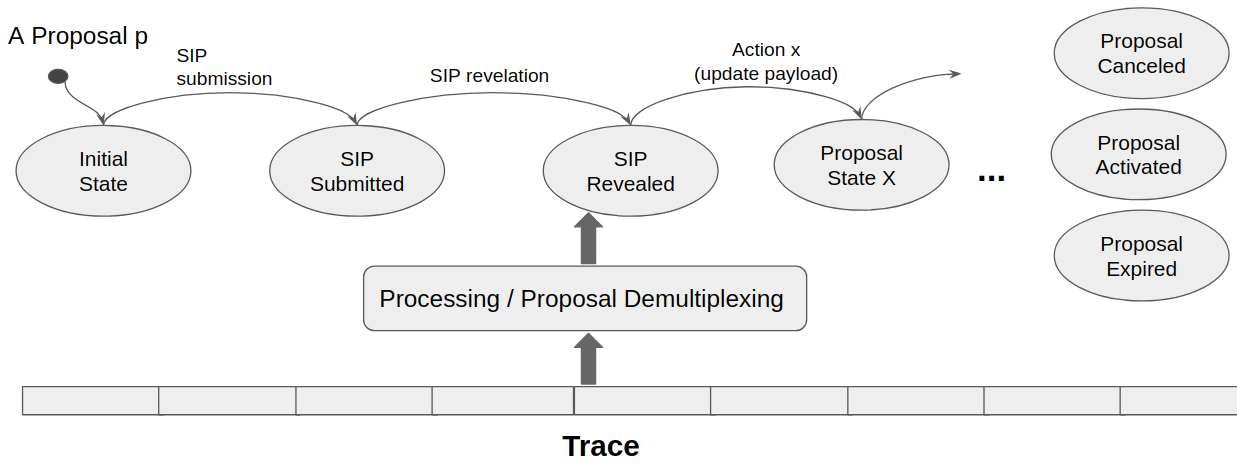
\includegraphics[width=0.8\columnwidth,
	keepaspectratio]{figures/state_transitions.png}
	\caption{Valid State Transitions in the Software Update Lifecycle.}
	\label{fig:state_transitions}
\end{figure}

\subsection{Transparent and auditable}\label{sec:transp_auditable}
This requirement states that anybody should be able to answer \emph{when},
\emph{why}, and \emph{how} the system has
evolved the way it has. The evolution history of the system should be open to
everyone and form a \emph{globally-consistent tamper-evident public release
	log}.

The first thing that we need to validate in this case is that the update events
are eventually stored in the blockchain. This will be the result of the
integration of the update system to Cardano. This validation criterion is
covered in
\ref{vc:Update_events_are_stored_in_the_Cardano_blockchain}, which checks
that the update protocol is transparent.

The second thing that we need to validate is auditability. To this end, we must
ensure that all the reported outcomes from the update system can eventually be
computed from the data stored on chain. This validation will be covered from
criteria~\ref{vc:votes_are_correctly_tallied} and
\ref{vc:Endorsements_are_correctly_tallied}. Note also that for all the 
on-chain 
data (i.e.,update payload), auditability is guaranteed by our update mechanism, 
however for the 
actual proposals (e.g., implementation code) that are stored off-chain, 
auditability is ensured only under 
the assumption that the utilized P2P storage system guarantees data 
availability.


\subsection{Secure activation}\label{sec:secure_act}
For this requirement we need to  define what is a \emph{secure
	activation} and validate that our protocol enables such an activation. The
formal definition of secure activation on blockchain systems can be found in
our paper \cite{secure_activation}. In summary, in order for an activation of
changes, which will enable the transition from a ledger $L_1$ to a ledger $L_2$,
to be secure the following properties must hold:
\begin{itemize}
	\item The updated ledger $L_2$ enjoys the \emph{liveness} property
	\item The updated ledger $L_2$ enjoys the \emph{consistency} property
	\item $L_2$ includes $L_1$ as a prefix.
\end{itemize}

The first two properties ensure that $L_2$ is indeed a secure ledger. This
means that if we were to start running $L_2$ from scratch then these two
properties would be enough to guarantee the security of the blockchain
protocol. The main prerequisite for this to be true, i.e., for $L_2$ to enjoy
liveness and consistency and thus to be secure, is to ensure that the
\emph{security assumption} $A_2$ of the $L_2$ protocol holds. In our update
protocol, this is guaranteed via the \emph{adoption threshold}. The definition
of the adoption threshold embeds ``the logic'' that enough honest parties must
have signaled upgrade readiness, before we allow the activation of changes to
take place. ``Enough'' here means with respect to the security assumption $A_2$.

The third property has to do with the fact that $L_2$ is not a new ledger
running from scratch, but it should be a valid \emph{continuation} of the
previous ledger $L_1$. This very important from a security
perspective since it ensures that all fund transfers made in the past are still
valid and the state of ledger $L_1$ will not just get wiped out at the hard
fork point to $L_2$. Thus we must guarantee that during the transition from
$L_1$ to
$L_2$, history is preserved. The secure activation protocol 
that we use in order to make a secure transition from $L_1$ to 
$L_2$, will be described in the forthcoming deliverable D3.3 ``Revision 
of Extended Core Protocols''.

All in all, in order to ensure the said secure activation properties, we define
the following validation criteria, which we detail next.
\begin{itemize}
	\item The adoption threshold is honored
	\item The update system preserves history across hard fork boundaries
\end{itemize}

\subsubsection{The adoption threshold is
	honored}\label{vc:The_adoption_threshold_is_honored}
The adoption threshold is the threshold used during the endorsement period (see
section \ref{sec:su_lifecycle}). When the stake endorsing a candidate proposal
is above this threshold, then we can be sure that enough honest parties have
signaled upgrade readiness and thus the security assumption of the upgraded
ledger
will hold upon activation. This validation requirement is covered by the
validation criterion \ref{vc:Decisions-are-honored-by-the-protocol}. Indeed, in
this criterion we validate that all proposals that have reached the state of
\emph{Activated}, they must have been previously approved. This means that
enough endorsements with respect to the adoption threshold have been submitted
by the block issuers.

In summary, in all generated traces and for all candidate
proposals that have reached the status of \emph{Activated}, there should be
endorsement stake previously submitted that exceeds the adoption threshold.
This result must be able to be computed from the data on the trace and thus
justify the transition of the candidate proposal to the activation state.

\subsubsection{The update system preserves history across hard fork
	boundaries}\label{vc:The_update_system_preserves_history_across_hard_fork_boundaries}
In this criterion we need to validate that after the update system gives the
green light for an activation - based on the adoption threshold discussed
before- the ledger stays intact, before and after the hard fork slot. We should
observe ledger 1 ($L_1$) before the hard fork slot and ledger 2 ($L_2$) after. 
This criterion
requires the integration with the Cardano ledger layer. In this integrated
version of our update protocol we will observe the ledger transitioning from
the previous version to the new one. It is essentially the validation criterion
\ref{vc:The-update-system-runs-on-Cardano}.

In summary, on the integrated (with Cardano) version of the
update system, we provide appropriate update payload that will update the
ledger from $L_1$ (version 1) to $L_2$ (version 2). We should be able to 
observe this
transition at the hard fork slot (epoch boundary) and validate that the ledger
forms a continuous and valid historical record of transactions regardless of
the version update. To this end, we must show that the first block of
the new version, will eventually stabilize and also that it ''points'' to a
stable block of the previous protocol version. The secure activation protocol 
that we use in order to make a secure transition from the previous version to 
the new one, will be described in the forthcoming deliverable D3.3 ``Revision 
of Extended Core Protocols''.

\subsection{Performant and scalable}\label{sec:perf_scalable}
This requirement is about showing that the update mechanism should not
impact negatively the performance of the underlying blockchain. For evaluating
the performance of the blockchain we utilize the following measures:
\begin{itemize}
	\item Transaction bytes per second (TBPS)
	\item Processing time and
	\item Memory usage
\end{itemize}
Finally, the update mechanism must be scalable. This means that as the number
of participants in the update protocol increases and eventually reaches the
scale of a global blockchain system, the update mechanism resource consumption
should scale up efficiently, i.e., ideally linearly to the number of
participants.
To validate all the above we define the following validation criteria:
\begin{itemize}
	\item Transaction throughput is not significantly affected.
	\item Low-impact on processing time.
	\item Low-impact on memory usage.
	\item The system should scale.
\end{itemize}

We detail each one next.

\subsubsection{Transaction throughput is not significantly
	affected}\label{vc:Transaction_throughput_is_not_significantly_affected}
An important measurement of a blockchain system’s performance is the number of
\emph{transaction bytes per-second (TBPS)} it can sustain. Unlike the more
commonly used metric, transactions per-second, this number is not dependent on
the chosen size of a transaction (which would allow to manipulate it at will by
choosing different transactions sizes). Running an update mechanism on the
blockchain should not result in a substantial performance degradation.
Therefore, in this validation criterion, we estimate the impact on performance
that the proposed update mechanism will have on a system’s TBPS. Our
estimations should be based on \emph{worst case scenarios}, which
determine upper bounds for the performance impact of the update mechanism.

The amount of data required by the update payload associated to a proposal
should be have little impact on the blockchain protocol. 
%The size of the update payload should be calculated and compared against the 
%system's TBPS. The size of the former relative to the latter should be 
%negligible. 
A worst case
analysis should be made that shows the TBPS impact of a proposal
as a function of the following variables:
\begin{itemize}
	\item Number of participants
	\item Number of voting rounds
	\item Duration of the update process
\end{itemize}

Different systems will have different requirements on the maximum TBPS impact
that they can tolerate. The aforementioned function should provide an easy way
to determine whether they can accommodate the additional usage requirements of
the update protocol. In practice, we will validate what percent of the
available TBPS throughput is consumed by the update mechanism and how this
percent scales as the number of participants increases.

\subsubsection{Low-impact on processing
	time}\label{vc:Low-impact_on_processing_time}
The processing time required by a node that runs the update protocol should not
be significantly impacted by the it. The bottlenecks of the protocol should be
identified, and for each one of them:
\begin{itemize}
	\item an asymptotic time complexity analysis should be made, which should
	provide	the resource requirements in terms of processing time.
	\item micro-benchmarks should be run that show the CPU time required for
	the most CPU-intensive parts of the update protocol, as a
	function of
	the input size. The benchmarks results should show that the processing time
	will not affect overall processing time of a node, assuming a reasonable
	input size.
	
\end{itemize}

\subsubsection{Low-impact on memory usage}\label{vc:Low-impact_on_memory_usage}
The memory usage requirements to store the update payload should be analyzed.
As with the previous validation criterion, micro-benchmarks should be executed
that show the consumption of memory by the update protocol. Memory usage should
be as small as possible (given the amount of data being manipulated by the
protocol).

\subsubsection{The system should scale}\label{vc:The_system_should_scale}
The resource consumption required by the update protocol should scale up
linearly with the number of participants. The results obtained in the previous
requirements can be used to demonstrate a linear relation between number of
participants and resource consumption (CPU, memory, impact in TBPS).

\subsection{Metadata driven}\label{sec:metadata_driven}
Metadata are very important in a software updates system, because they
provide the context of a software update. Without metadata all updates would
look the same. In our update protocol, the proposals should be able to specify
as part of its metadata the following information:

\begin{itemize}
	\item voting period length
	\item dependencies with other versions
	\item activation priority
	\item deployment window
\end{itemize}

and the protocol should make sure that these are honored as part of the update
logic implemented. The voting period duration corresponds to the voting
processes in the Ideation and Approval phases (see figure
\ref{fig:su_lifecycle}) in the lifecycle of a software update and is attached
to the submission of SIPs and UPs respectively. It is the number of slots
during which votes are accepted for a specific proposal. Dependencies refer to
the protocol version upon which an update is based. It is the version that a
specific update is compatible with and can be safely deployed on (i.e., the
version that an update supersedes). Priorities are declared in the proposal's
metadata in the form of software versions. Since the update system guarantees
that the protocol versions can only strictly increase, the lower the version
is, the higher is the priority of a proposal. Ultimately, the community
decides (through the available voting processes), which proposal will move
forward, in the case of proposals with the same version (i.e., priority).
Finally the deployment window, which is also called \emph{safety lag}, is
defined in number of epochs and it is a safe time window that allows sufficient
time to stakeholders to download the update and upgrade their software.

The following validation criteria will validate if the update protocol
indeed honors the proposal's metadata.
\begin{itemize}
	\item The voting period length is honored
	\item Version dependencies are honored
	\item Priorities are honored
	\item The deployment window is honored
\end{itemize}
We detail these validation criteria next:

\subsubsection{The voting period length is honored}
\label{vc:The_voting_period_length_is_honored}

The update prototype should provide a mechanism for specifying the duration of
the voting period, and ensure that a proposal is granted the voting period
duration it specifies. Validation criterion
\ref{vc:votes_are_correctly_tallied} requires that the vote result that
computed over the generated trace of events is the same as the result reported
by the system. In this computation, we will use the voting period defined in
the proposal's metadata. If the update system does not honor the voting
duration in the metadata, our property-tests should find a case in which
comparison will fail. Therefore this validation criteria is subsumed in
validation criteria~\ref{vc:votes_are_correctly_tallied}.

\subsubsection{Version dependencies are honored}
\label{vc:Version_dependencies_are_honored}
The update prototype should provide a mechanism for specifying version
dependencies, and ensure that a protocol update should always be applied to a
protocol version that it depends on. This validation criterion will ensure that
every update is applied only on the version that (based on its metadata) it
supersedes. As we mentioned earlier, in our prototype every software update
supersedes one and only one protocol version.

In summary, for all trace of events generated, and for all
updates that have been activated superseding a version $X$, $X$ should match
the dependency version (i.e., to be superseded) specified in the corresponding
metadata of the said update.

\subsubsection{Priorities are honored}\label{vc:Priorities_are_honored}
The update protocol should provide a way for update proposals to specify their
priority, and once updates get enough endorsements, they should be activated
according to their priority. As we mentioned earlier, priorities are defined by
means of software versions. The lower the version, the higher the priority.
Protocol versions increase monotonically. This validation criterion will ensure
that updates are activated based on their (metadata-defined) priorities, which
are of course confirmed by the stakeholders approval.

In summary, for all generated traces of events and for all
updates activated, two conditions must hold:
\begin{itemize}
	\item The version that the system upgrades to, coincides with the version
	of the update defined in the metadata
	\item The versions of the system increase monotonically
\end{itemize}

\subsubsection{The deployment window is honored}
\label{vc:The_deployment_window_is_honored}

The update protocol should ensure that each proposal in the endorsement period
(see section \ref{sec:su_lifecycle}) is allowed to have the endorsement window
that this proposal specifies. The endorsement window is specified in number of
epochs and defines the time window during which participants can upgrade their
software and signal (i.e., endorse) their upgrade readiness (see note on
endorsements in  section \ref{vc:endorsements_not_rejected}).
%
As in the case of the validation
criteria in section ~\ref{vc:The_voting_period_length_is_honored}, the tests 
will compute
(and thus double check) the results of an endorsement period. If there is a
discrepancy between the proposal-specified deployment window and the deployment
window allowed by the system, then the property tests should find a case in
which the two endorsement-tally results do not match. Therefore, this
validation criteria is subsumed in validation
criteria~\ref{vc:Endorsements_are_correctly_tallied}.

\subsection{Update logic consistency}\label{sec:update_logic}
The update system must implement an \emph{update logic} that handles software
dependencies, update priorities, software conflicts, and emergencies in a
smooth way that always guarantees the \emph{consistency} of the blockchain
software.

In our prototype, every software update supersedes one and only one protocol
version. This is the version that it \emph{depends} on. Moreover, every update
has a version. It is the to-be version of the protocol after the update is
activated. Our update mechanism ensures that protocol versions
increase strictly-monotonically. In our model, we allow only a single base
version per-update proposal. A conflict is the case where two updates are
applied on the same base version. The update mechanism implements an update
logic that resolves such conflicts and allows only a single proposal to
supersede the current version each time.

Priorities are defined by means of software versions. The lower the version,
the higher the priority. In the case of multiple updates with the same
priority,
the community is the ultimate decision maker of which one will move forward to
the next phase. If two proposals with the same version are in the approval
phase and both are approved, then the last one entering the activation phase,
will survive. In the unlikely case, where the two proposals coincide in their
voting period  ends and thus are approved at the very same slot, then we
resolve this conflict by choosing the one with the higher stake in favor to
enter the activation queue. In the even more unlikely case, where both have the
same stake in favor, then we choose the proposal with the greatest id (proposal
hash) to enter the activation queue.

Emergency handling is realized by means of \emph{cancellations}. A
proposal can be explicitly canceled. This allows the experts and community to
cancel an approved implementation after a (significant) problem with it was
discovered. An explicit cancellation is submitted as a SIP that must justify
the reason for canceling the proposals. When submitted as an update proposal
(UP), the cancellation must specify the proposals that it will cancel if
approved. The explicit cancellation also goes through the ideation and approval
phases, however, the explicit cancellation immediately cancels the proposals it
refers to once it gets approved by the expert pools in the approval phase.
Cancellation proposals have no next-versions associated with it. They only
specify the hash of the implementations they cancel.

If the candidate proposal already got the required endorsements (which means 
that the
cancellation arrived at or later than the slot at which the tally occurred, 
this is 2k blocks before
the end of an epoch), and is waiting to be activated, then the cancellation 
update cannot stop it. In this case, a new software update must be implemented 
and submitted that will correct the identified problem. Nodes that upgraded to 
a canceled version can continue to operate normally following
the current version since the upgraded version must be able to follow the 
current ledger and
consensus rules. Then it is up to the node operators to revert back to the 
previous version, or
continue using the software version that can also validate the protocol version 
that got discarded.
The ledger rules shall ensure that this discarded protocol version is never 
applied.


The following validation criterion ensures that update system implements a
consistent update logic and is detailed next.

\subsubsection{Consistent update logic}\label{vc:consistent_update_logic}
The update protocol should implement a consistent update logic. This means that
it handles dependencies, conflicts and priorities in such a way that the
blockchain software always reaches a consistent state. In particular, the
protocol should allow a proposal to be activated if and
only if:
\begin{itemize}
	\item is approved,
	\item meets its dependencies,
	\item does not conflict with the current version,
	\item has the highest priority among competing proposals, and
	\item receives enough endorsements.
\end{itemize}

In summary, for all traces generated and for all proposals
activated the above validity conditions should hold. In addition, carefully 
selected unit tests will validate the correctness of the cancellation mechanism.

\subsection{Validation criteria summary}\label{sec:val_criteria_summary}
In table \ref{table:all_val_criteria}, we summarize all the aforementioned 
validation criteria. In the leftmost column, we present the high-level 
requirements, or vision statements. Validation criteria are grouped in four 
different categories:
\begin{itemize}
	\item \textbf{Liveness}: criteria that ensure that something 
	''good'' eventually happens.
	\item \textbf{Safety}: criteria that ensure that nothing 
	''bad'' happens.
	\item \textbf{Performance}: criteria that validate the performance and 
	scalability of the update mechanism
	\item \textbf{Integration}: criteria that validate the integration with the 
	Cardano blockchain system.
\end{itemize}


\begin{center}
	\tablefirsthead{%
		\hline
		\multirow{2}{8em}{			
			\textbf{Vision Statements}
		} 
		&
		\multicolumn{4}{c|}{\textbf{Validation Criteria}} \\
		
		& Liveness & Safety & Performance & Integration \\
		\hline \hline				
	}
	\tablehead{%
		\hline
		\multicolumn{5}{|l|}{\small\sl continued from previous page}\\
		\hline
		\multirow{2}{8em}{\textbf{Vision Statements}} &
		\multicolumn{4}{c|}{\textbf{Validation Criteria}} \\
		
		& Liveness & Safety & Performance & Integration \\
		\hline \hline
	}
	\tabletail{%
		\hline
		\multicolumn{5}{|r|}{\small\sl continued on next page}\\
		\hline}
	\tablelasttail{\hline}
	\bottomcaption{Summary of all validation criteria.}
	\label{table:all_val_criteria}	
\end{center}

\pagestyle{empty}
\begin{landscape}
	%\begin{table}[htbp]
	\begin{center}
		\begin{supertabular}{|p{0.15\linewidth} | 
				p{0.2\linewidth}|p{0.2\linewidth} | 
				p{0.2\linewidth}|p{0.2\linewidth} | }
			%				\hline
			%				Vision Statements & Liveness & Safety & Performance 
			%& 
			%				Integration \\
			%				\hline \hline
			\multirow{5}{8em}{Open Participation Enabled} & 
			&
			\ref{vc:proposals_authorship} Authorship of proposals should be 
			preserved & 				
			& \\
			
			& 
			&
			\ref{vc:commits_not_rejected} Valid proposal commitments 
			are not 
			rejected & 				 
			& \\
			
			& 
			&
			\ref{vc:revelations_not_rejected} Valid proposal revelations 
			are not rejected & 				 
			& \\
			
			& 
			&
			\ref{vc:votes_not_rejected} Valid proposal votes are not 
			rejected & 				 
			& \\
			
			& 
			&
			\ref{vc:endorsements_not_rejected} Valid implementation 
			endorsements are not rejected & 				 
			& \\
			\hline
			
			\multirow{2}{10em}{Decentralized Decision-Making Enabled} & 
			\ref{vc:Decisions-are-honored-by-the-protocol} Decisions are 
			honored by the protocol &
			\ref{vc:votes_are_correctly_tallied} Votes are correctly 
			tallied	& 				
			& \\
			
			& 
			&
			\ref{vc:Endorsements_are_correctly_tallied} Endorsements are 
			correctly tallied & 				 
			& \\
			
			\hline
			\multirow{2}{10em}{Protocol-Driven} & 
			\ref{vc:Update_events_are_stored_in_the_Cardano_blockchain} 
			Update events are eventually stored in the Cardano blockchain &
			& 				
			& 
			\ref{vc:The-update-system-runs-on-Cardano} The update system 
			runs on Cardano
			\\
			
			& 
			&
			\ref{vc:The_proposal_state_transitions_should_be_specified_and_verified}
			The proposal state transitions should be specified 
			and verified & 				
			& 
			\ref{vc:The-update-protocol-works-as-expected-in-Cardano} The 
			update protocol works as expected in Cardano
			\\
			
			\hline
			\multirow{2}{10em}{Transparent and Auditable} & 
			\ref{vc:Update_events_are_stored_in_the_Cardano_blockchain} 
			Update events are eventually stored in the Cardano blockchain &
			\ref{vc:votes_are_correctly_tallied} Votes are correctly 
			tallied	& 				
			& 
			\\
			
			&
			&
			\ref{vc:Endorsements_are_correctly_tallied} Endorsements are 
			correctly tallied & 				 
			& \\
			
			\hline
			\multirow{1}{10em}{Secure Activation Enabled} & 				
			\ref{vc:The_update_system_preserves_history_across_hard_fork_boundaries}
			 The 
			update system preserves history across hard fork boundaries &
			\ref{vc:The_adoption_threshold_is_honored}  The adoption 
			threshold is honored 
			& &
			\\
			
			%\hline
			\multirow{4}{8em}{Performant and Scalable} & 
			&
			& 				
			\ref{vc:Transaction_throughput_is_not_significantly_affected} 
			Transaction throughput is not significantly affected & 
			\\
			
			& 
			&
			& 				
			\ref{vc:Low-impact_on_processing_time} 
			Low-impact on processing time & 
			\\
			
			& 
			&
			& 				
			\ref{vc:Low-impact_on_memory_usage} 
			Low-impact on memory usage & 
			\\
			
			& 
			&
			& 				
			\ref{vc:The_system_should_scale} 
			The system should scale & 
			\\
			
			\hline
			\multirow{4}{8em}{Metadata-Driven Update Logic} & 
			\ref{vc:consistent_update_logic} Consistent update logic		
			&
			\ref{vc:The_voting_period_length_is_honored} The voting period 
			length is honored
			& 				
			& 
			\\
			
			& 
			&
			\ref{vc:Version_dependencies_are_honored} Version dependencies 
			are honored
			& 				
			& 
			\\
			
			& 
			&
			\ref{vc:Priorities_are_honored} Priorities are honored
			& 				
			& 
			\\
			
			& 
			&
			\ref{vc:The_deployment_window_is_honored} The deployment window 
			is honored
			& 				
			& 
			\\
			
			\hline
		\end{supertabular}
	\end{center}
	%	\caption{Summary of all validation criteria.}
	%	\label{table:all_val_criteria}	
	%	\end{table}
\end{landscape}
\pagestyle{plain}

\subsection{Validation Results}\label{validation_results}